%!TEX program = xelatex
\documentclass[cn,hazy,blue,14pt,screen]{elegantnote}
\title{计算机基础知识培训}

\author{小布老师}
\institute{樱桃溪学院}

\version{0.10}
\date{\zhdate{2025/03/28}}

\usepackage{array}

\begin{document}

\maketitle

\centerline{
  \includegraphics[width=0.2\textwidth]{clublogo.jpg}
}

\section{基本概念 - 十进制(decimal)}
\begin{itemize}
  \item 逢十进一,包含0,1,2,3,4,5,6,7,8,9共计10个基本数字。 
  \item 人类算数采用十进制,可能跟人类有十根手指有关。它是世界上应用最广泛的进位制。
  \item 一个十进制数d的大小,除了取决于它包含的基本数字,还和这些数字的位置相关。
  \item 例如:315 = (3 * 100) + (1 * 10) + (5 * 1)
\end{itemize}

\begin{center}
	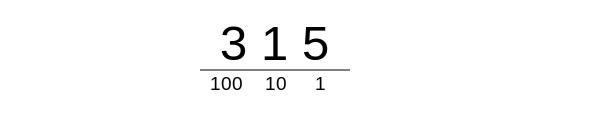
\includegraphics[width=0.9\textwidth]{x0008.pdf}
	\captionof{figure}{一个十进制数}
\end{center}

\newpage

\section{基本概念 - 二进制(binary)}
\begin{itemize}
  \item 逢二进一,包含0,1共计2个基本数字,这两个基本数字被称为“比特(bit)”。 
  \item 一个二进制数b的大小,除了取决于它包含的基本数字,还和这些数字的位置相关。
  \item 例如:1101 = (1 * 8) + (1 * 4) + (0 * 2) + (1 * 1) = 13(十进制)
\end{itemize}

\begin{center}
	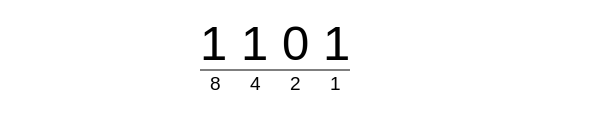
\includegraphics[width=0.9\textwidth]{x0009.pdf}
	\captionof{figure}{一个二进制数}
\end{center}

\newpage

\section{基本概念 - 十六进制(hexadecimal/hex)}
\begin{itemize}
  \item 逢十六进一,包含0 - 9和A、B、C、D、E、F共计16个基本数字。 
  \item 一个十六进制数h的大小,除了取决于它包含的基本数字,还和这些数字的位置相关。
  \item 例如:C5 = (12 * 16) + (5 * 1) = 197(十进制)
\end{itemize}

\begin{center}
	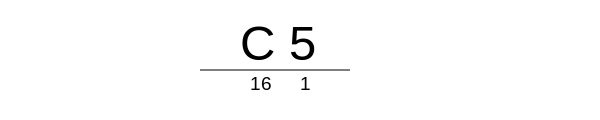
\includegraphics[width=0.9\textwidth]{x0010.pdf}
	\captionof{figure}{一个十六进制数}
\end{center}

\newpage

\section{十进制、二进制和十六进制之间的转换}
\begin{itemize}
  \item 我们把四位二进制作为一个转换的基本单元,如1011,0110等。 
\end{itemize}

\begin{center}
	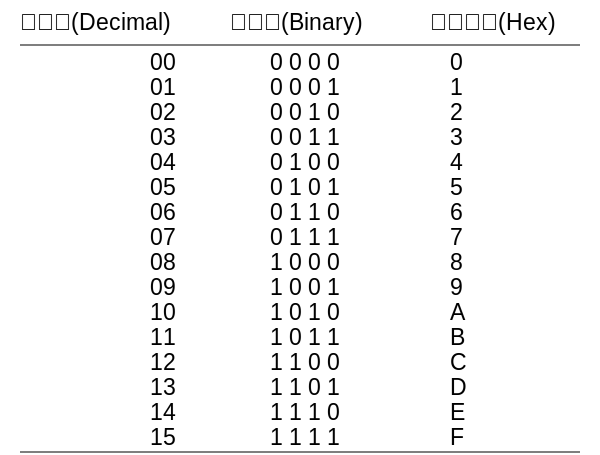
\includegraphics[width=0.6\textwidth]{x0007.pdf}
	\captionof{figure}{十进制、二进制和十六进制之间的转换}
\end{center}

\newpage

\section{基本概念 - 比特(bit)和字节(byte)}

\begin{itemize}
  \item \textbf{比特(bit)}:亦称二进制位,指二进制中的一位,是信息的最小单位,其取值为0或者1。
  \item \textbf{字节(byte)}:由8个比特组成的一个组,即一个字节为8比特。
\end{itemize}

\begin{center}
	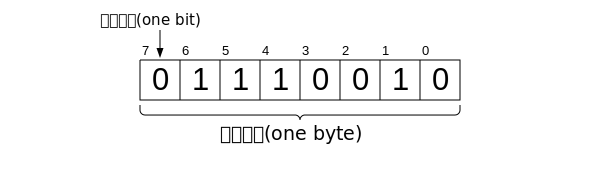
\includegraphics[width=0.9\textwidth]{x0005.pdf}
	\captionof{figure}{bit和byte的概念示意图}
\end{center}

\newpage
%%%%%%%%%%%%%%%%%%%%%%%%%%%%%%%%%%%%%%%
\section{ASCII(American Standard Code for Information Interchange)表}
\begin{center}
	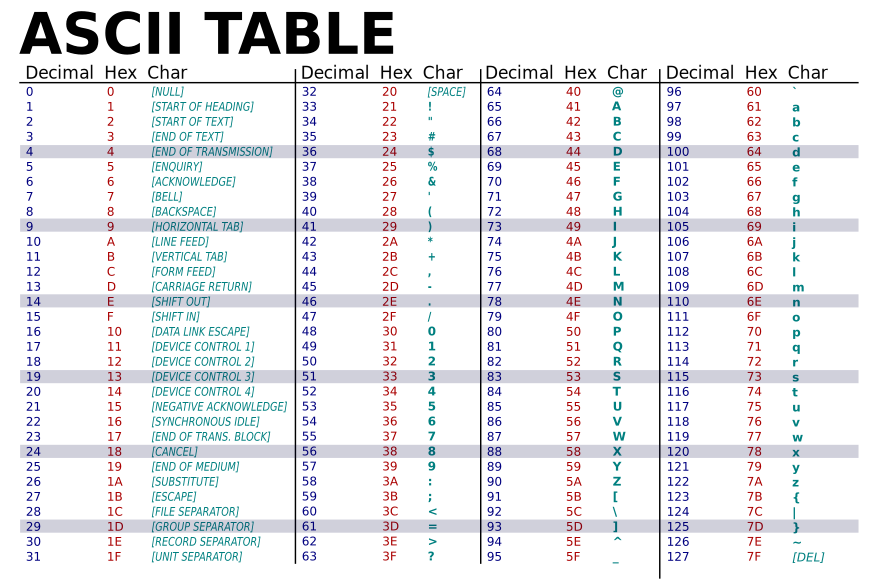
\includegraphics[width=0.9\textwidth]{x0011.pdf}
	\captionof{figure}{ASCII表}
\end{center}

\newpage
%%%%%%%%%%%%%%%%%%%%%%%%%%%%%%%%%%%%%%%

\section{UTF-8(8-bit Unicode Transformation Format)编码}
\begin{itemize}
  \item UTF-8是一种针对Unicode的可变长度字元编码。
  \item 它用一至四个字节对Unicode字符集中的所有有效编码点进行编码,属于Unicode标准的一部分。
  \item 自2009年以来,UTF-8一直是万维网的最主要的编码形式。
\end{itemize}

\begin{center}
	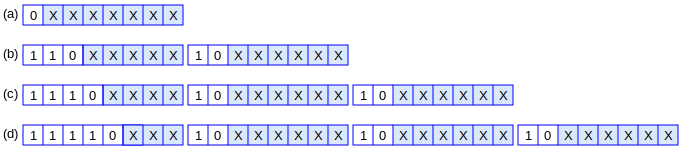
\includegraphics[width=0.9\textwidth]{x0012.pdf}
	\captionof{figure}{UTF8编码}
\end{center}

\newpage

\section{计算机的基本结构}

\begin{center}
	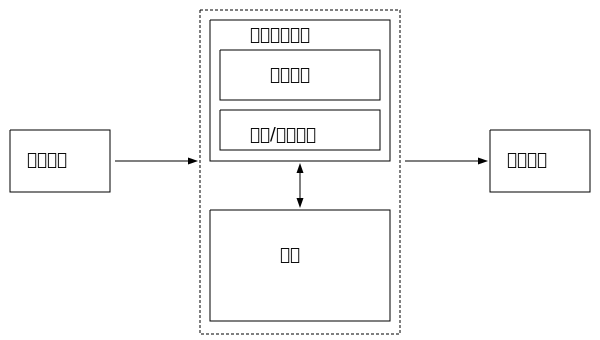
\includegraphics[width=0.9\textwidth]{x0014.pdf}
	\captionof{figure}{计算机的基本结构}
\end{center}
\newpage
%%%%%%%%%%%%%%%%%%%%%%%%%%%%%%%%%%%%%%%%%%%%%%%%%%%%%%%%%%%%

\section{计算机的基本结构}

\begin{itemize}
  \item \textbf{中央处理单元(CPU: Central Processing Unit)}:文件和内存均可用一个统一的抽象模型来表示。
  \item \textbf{内存(Memory)}:内存里保存的信息断电后就会消失,文件存储在磁盘上,其内容在断电后也不会消失。
  \item \textbf{输入设备(Input Device)}:内存里保存的信息断电后就会消失,文件存储在磁盘上,其内容在断电后也不会消失。
  \item \textbf{输出设备(Output Device)}:内存里保存的信息断电后就会消失,文件存储在磁盘上,其内容在断电后也不会消失。
  \item \textbf{控制单元(Control Unit)}:内存里保存的信息断电后就会消失,文件存储在磁盘上,其内容在断电后也不会消失。
  \item \textbf{数学/逻辑单元(Arithmetic/Logic Unit)}:内存里保存的信息断电后就会消失,文件存储在磁盘上,其内容在断电后也不会消失。
\end{itemize}

\newpage
%%%%%%%%%%%%%%%%%%%%%%%%%%%%%%%%%%%%%%%%%%%%%%%%%%%%%%%%%%%%

\section{基本概念 - 内存(memory)和文件(file)}

\begin{itemize}
  \item \textbf{内存和文件的共同点}:文件和内存均可用一个统一的抽象模型来表示,即:若干字节组成的有序队列,如下图所示,这个有序的字节序列由n个字节组成。“字节”是绝大多数计算机体系结构中最小的可寻址内存单元。
  \item \textbf{内存和文件的不同点}:内存里保存的信息断电后就会消失,文件存储在磁盘上,其内容在断电后也不会消失。
\end{itemize}

\begin{center}
	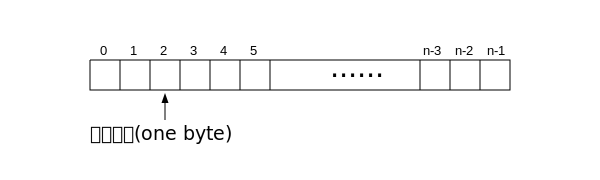
\includegraphics[width=0.9\textwidth]{x0006.pdf}
	\captionof{figure}{memory和file的概念示意图}
\end{center}
\newpage

%%%%%%%%%%%%%%%%%%%%%%%%%%%%%%%%%%%%%%%%%%%%%%%%%%%%%%%%%%%%
\section{计算机的层次结构}

\begin{center}
	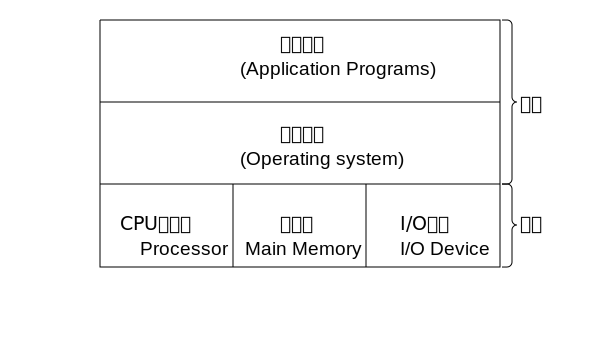
\includegraphics[width=0.9\textwidth]{x0015.pdf}
	\captionof{figure}{计算机的基本结构}
\end{center}
\newpage
%%%%%%%%%%%%%%%%%%%%%%%%%%%%%%%%%%%%%%%%%%%%%%%%%%%%%%%%%%%%

\section{黑客工具hexdump}
\begin{lstlisting}
ubuntu@mylab:~/wilson/clang$ ls -l
total 4
-rw-rw-r-- 1 ubuntu ubuntu 103 Mar 29 20:17 hello.c

ubuntu@mylab:~/wilson/clang$ cat hello.c
#include <stdio.h>

int main(int argc, const char* argv[])
{
        printf("Hello, world!\n");
        return 0;
}

ubuntu@mylab:~/wilson/clang$ hexdump -C hello.c
00000000  23 69 6e 63 6c 75 64 65  20 3c 73 74 64 69 6f 2e  |#include <stdio.|
00000010  68 3e 0a 0a 69 6e 74 20  6d 61 69 6e 28 69 6e 74  |h>..int main(int|
00000020  20 61 72 67 63 2c 20 63  6f 6e 73 74 20 63 68 61  | argc, const cha|
00000030  72 2a 20 61 72 67 76 5b  5d 29 0a 7b 0a 09 70 72  |r* argv[]).{..pr|
00000040  69 6e 74 66 28 22 48 65  6c 6c 6f 2c 20 77 6f 72  |intf("Hello, wor|
00000050  6c 64 21 5c 6e 22 29 3b  0a 09 72 65 74 75 72 6e  |ld!\n");..return|
00000060  20 30 3b 0a 7d 0a 0a                              | 0;.}..|
00000067
\end{lstlisting}

\newpage
%%%%%%%%%%%%%%%%%%%%%%%%%%%%%%%%%%%%%%%%%%%%%%%%%%%%%%%%%%%%
\section{C语言程序的编译过程}
\begin{center}
	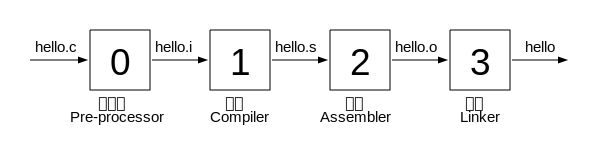
\includegraphics[width=0.9\textwidth]{x0013.pdf}
	\captionof{figure}{C语言程序的编译过程}
\end{center}
\newpage
%%%%%%%%%%%%%%%%%%%%%%%%%%%%%%%%%%%%%%%%%%%%%%%%%%%%%%%%%%%%

\end{document}
